\section*{Ejercicio 01 - Teclado Random}

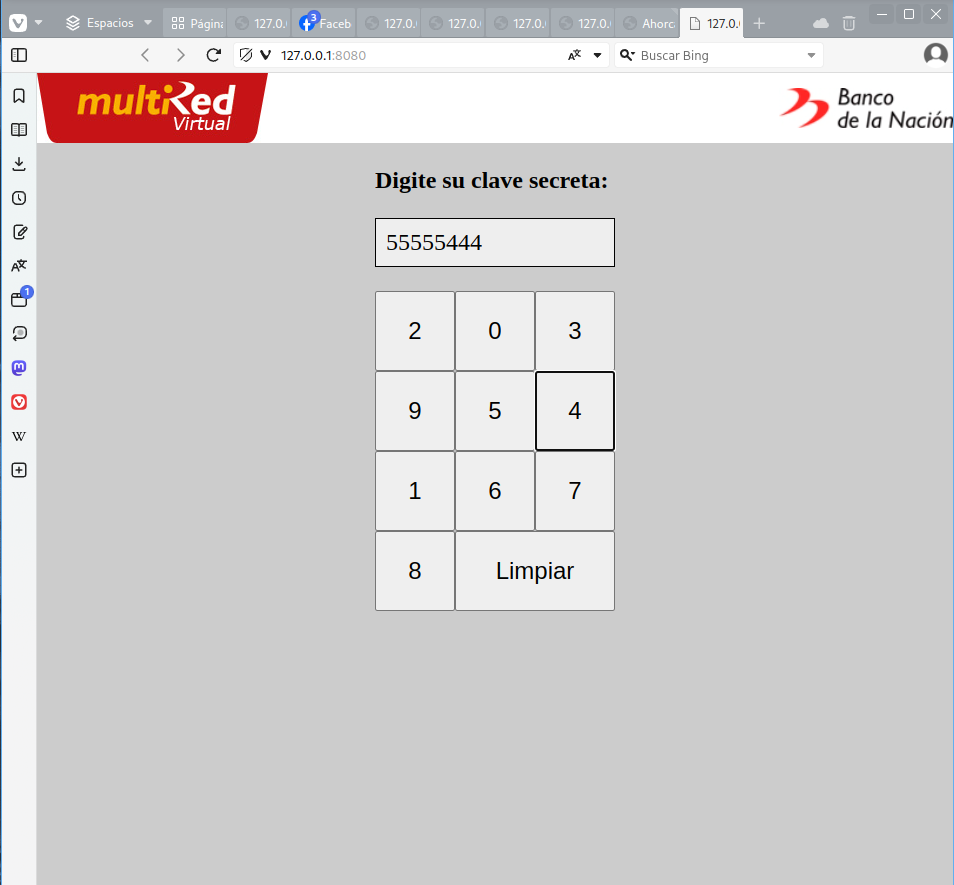
\includegraphics[width=0.5\textwidth]{./img/ejercicio01.png}

Este informe detalla la creación y configuración de un documento HTML dinámico utilizando JavaScript puro. El código tiene como objetivo generar una interfaz de usuario (UI) que incluye una barra de navegación con dos logotipos y un área principal que contiene un campo de entrada de texto simulado y un teclado numérico aleatorio. A continuación, se explica cada parte del código con porciones de código relevantes.

\subsection*{Creación de la Barra de Navegación}

Primero, se crea un elemento \texttt{nav} y se agregan dos imágenes de logotipos a esta barra de navegación.

\begin{lstlisting}[language=JavaScript]
let nav = document.createElement("nav");

let logo = document.createElement("img");
logo.src = "./img/logo-multired.jpg";
nav.appendChild(logo);

let logo2 = document.createElement("img");
logo2.src = "./img/Logo_BN.jpg";
logo2.style.height = "40px";
logo2.style.width = "auto";
logo2.style.alignSelf = "center";
nav.appendChild(logo2);
\end{lstlisting}

En esta parte del código, se crean los elementos \texttt{nav} y \texttt{img} utilizando \texttt{document.createElement}. Los atributos de las imágenes (como \texttt{src} y estilos) se definen y las imágenes se añaden como hijos del elemento \texttt{nav}.

\subsection*{Estilos para la Barra de Navegación}

Luego, se aplican estilos CSS al \texttt{nav} para estructurarlo visualmente.

\begin{lstlisting}[language=JavaScript]
nav.style.display = "flex";
nav.style.justifyContent = "space-between";

document.body.appendChild(nav);
\end{lstlisting}

Se utiliza \texttt{style} para establecer la propiedad \texttt{display} como \texttt{flex}, lo que permite una distribución flexible de los elementos hijos, y \texttt{justifyContent} para espaciar los elementos (los logotipos) uniformemente.

\subsection*{Creación del Área Principal}

A continuación, se crea el elemento \texttt{main} y un contenedor \texttt{div} dentro de él.

\begin{lstlisting}[language=JavaScript]
let main = document.createElement("main");
document.body.appendChild(main);

let mainDiv = document.createElement("div");
main.appendChild(mainDiv);
\end{lstlisting}

\subsection*{Adición de la Etiqueta y Campo de Entrada}

Dentro del \texttt{div} principal, se agrega un \texttt{p} para la etiqueta y otro \texttt{p} para simular el campo de entrada de texto.

\begin{lstlisting}[language=JavaScript]
let label = document.createElement("p");
label.textContent = "Digite su clave secreta:";
label.style.fontSize = "1.5rem";
label.style.fontWeight = "bold";
mainDiv.appendChild(label);

let camp = document.createElement("p");
camp.style.fontSize = "1.5rem";
mainDiv.appendChild(camp);
camp.style.minHeight = "1.5rem";
camp.style.padding = "10px 10px";
camp.style.border = "1px solid black";
camp.style.backgroundColor = "#eee";
camp.style.display = "flex";
camp.style.alignContent = "center";
camp.style.overflow = "hidden";
\end{lstlisting}

Estos elementos de párrafo (\texttt{p}) se estilizan para parecer un campo de entrada de texto. El campo de entrada (\texttt{camp}) tiene estilos adicionales para simular un área de entrada segura.

\subsection*{Función para Mezclar los Números}

Se define una función \texttt{shuffle} para mezclar un array de números, que se usará para crear el teclado numérico aleatorio.

\begin{lstlisting}[language=JavaScript]
function shuffle(array) {
  for (let i = array.length - 1; i > 0; i--) {
    const j = Math.floor(Math.random() * (i + 1));
    [array[i], array[j]] = [array[j], array[i]];
  }
  return array;
}

let numbers = Array.from({ length: 10 }, (_, i) => i); 
numbers = shuffle(numbers); 
\end{lstlisting}

La función \texttt{shuffle} utiliza el algoritmo de Fisher-Yates para mezclar los elementos de un array.

\subsection*{Creación del Teclado Numérico}

El teclado numérico se crea como un \texttt{div} y se añaden botones numerados, incluyendo un botón de "Limpiar".

\begin{lstlisting}[language=JavaScript]
let keyboard = document.createElement("div");

for (let i = 0; i <= 10; i++) {
  let key = document.createElement("button");
  let name = i < 10 ? numbers[i] : "Limpiar"; 
  if (i == 10) {
    key.style.gridColumn = "span 2";
  }
  key.textContent = name;
  key.style.height = "80px";
  keyboard.appendChild(key);
  key.addEventListener("click", () => {
    if (name == "Limpiar") {
      camp.textContent = "";
      return;
    }
    camp.textContent += name;
  });
  key.style.fontSize = "1.5rem";
}

mainDiv.appendChild(keyboard);
\end{lstlisting}

Cada botón tiene un \texttt{event listener} que actualiza el campo de entrada (\texttt{camp}) con el número correspondiente o lo limpia si se presiona "Limpiar".

\subsection*{Estilos Adicionales para el Documento y los Elementos}

Se aplican estilos globales y específicos a varios elementos para asegurar una presentación consistente.

\begin{lstlisting}[language=JavaScript]
document.documentElement.style.margin = 0;
document.documentElement.style.padding = 0;
document.body.style.margin = 0;
document.body.style.padding = 0;

document.body.style.height = "calc(100vh - 70px)";
main.style.width = "100vw";
main.style.height = "calc(100vh - 70px)";
main.style.display = "flex";
main.style.backgroundColor = "#ccc";
main.style.justifyContent = "center";
main.style.alignContent = "center";

mainDiv.style.width = "240px";
mainDiv.style.height = "100px";

keyboard.style.display = "grid";
keyboard.style.gridTemplateColumns = "1fr 1fr 1fr";
\end{lstlisting}

Estos estilos aseguran que el documento ocupe toda la ventana del navegador, que el contenido principal esté centrado y que el teclado numérico esté distribuido en una cuadrícula de tres columnas.
